\section*{první mechanická varianta}
\addcontentsline{toc}{section}{první mechanická varianta}
První, čistě mechanická varianta, vznikla začátkem srpna 2019, chvíli po výše obšírněji popsané elektronické variantě.
Měla stále poměrně klasický vzhled trezoru, tedy zamykatelná skříňka, která obsahovala dvě kola, která ovládala možnost pohybu jednoduché západky.
Na rozdíl od jeho elektronického předchůdce bylo vše zajímavé uvnitř dveří. Také byla určená jako základ pro případný upgrade na elektronickou
variantu. Na podobné vylepšení mělo stačit odstranění kódovacích kol a přidělání elektronické části. Toto sice fungovalo obstojně, zároveň 
i jako motivace, ale kvůli pozdější změně konceptu mechanizmu tento nápad padl.
Tato varianta však nebyla, kvůli přílišným nárokům na přesnost, vhodná pro stavbu s malými dětmi, pro které byla určena jakožto předstupeň 
k variantě elektronické (která vyžaduje i znalosti, nebo alespoň ochotu k učení, programování).

\begin{figure}[htbp]
    \centering
    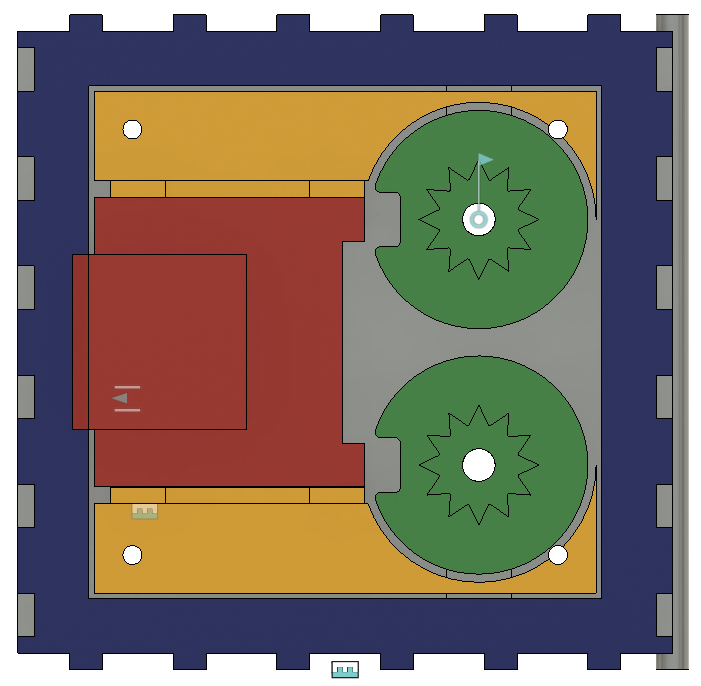
\includegraphics[width=260]{kapitoly/obrazky/M1/mechanizmus.png}
    \caption{zelená značí kódová kola, červená západku, modrá pevnou část trezoru(otvor) a žluté díly tvoří distanci}
    \label{fig:M1}
\end{figure}
\newpage